\documentclass[shadesubsections,compress,14pt,mathserif]{beamer}
\usepackage[danish]{babel}	
\usepackage{tikz,circuitikz}
\usetikzlibrary{shapes, positioning}
\usenavigationsymbolstemplate{}
\usepackage{xcolor,pgfplots}
\usepackage[absolute,overlay]{textpos}
\usepackage{amsthm,amsfonts}
%\usepackage[T1]{fontenc}
% \usepackage{fullpage}
% Dokumentets sprog
%\usepackage{mathtools}
%\usepackage{pxfonts}
\usepackage{eulervm}
\usepackage[export]{adjustbox}
\everymath{\color{purple}}
% Class options include: notes, notesonly, handout, trans,
%                        hidesubsections, shadesubsections,
%                        inrow, blue, red, grey, brown

% Theme for beamer presentation.
%\usepackage{beamertheme} 
% Other themes include: beamerthemebars, beamerthemelined, 
%                       beamerthemetree, beamerthemetreebars  
\newcommand{\minus}{\scalebox{0.5}[1.0]{\( - \)}}
\newcommand{\adv}{\ensuremath{\mathcal A}}
\newcommand{\F}{\ensuremath{{\mathbb F}}}
\newcommand{\G}{\ensuremath{{\mathbb G}}}
\renewcommand{\P}{\ensuremath{{\mathbb P}}}
\newcommand{\Z}{\ensuremath{{\mathbb Z}}\xspace}
\newcommand{\Fclosure}{\ensuremath{{\overline{\mathbb{F}}}_p}}
\newcommand{\set}[1]{\ensuremath{\left\{#1\right\}}}
\newcommand{\bin}{\ensuremath{\set{0,1}}}
\newcommand{\cube}{\ensuremath{\bin^n}}

\newcommand{\sett}[2]{\ensuremath{\left\{#1\right\}_{#2}}}
\newcommand{\enc}[1]{\ensuremath{\left[#1\right ]}}
% \newcommand{\kzg}[1]{\ensuremath{\enc{#1(x)}}}
\newcommand{\cm}{\ensuremath{\mathsf{cm}}}
\newcommand{\kzg}[1]{\cm(#1)}
\newcommand{\open}[1]{\ensuremath{\mathsf{open}(#1)}}
\newcommand{\verify}[1]{\ensuremath{\mathsf{verify}(#1)}}
\newcommand{\defeq}{\ensuremath{:=}}
\newcommand{\helper}{\ensuremath{\mathcal{H}}}
\newcommand{\ver}{\ensuremath{\mathcal{V}}}
\newcommand{\prv}{\ensuremath{\mathcal{P}}}
 \newcommand{\polysofdeg}[1]{\F_{< #1}[X]}
%  \newcommand{\endoss}{\ensuremath{\mathrm{END}_E}}
 \newcommand{\hl}[1]{\textbf{\textit{#1}}}
 \newcommand{\polys}{\F[X]}
\newcommand{\acc}{{\mathbf{acc}}}
\newcommand{\rej}{{\mathbf{rej}}}
\newcommand{\ideal}{\mathbf{I}}
\newcommand{\gen}{\alpha}
\newcommand{\spac}{\\  \vspace{0.2in} \noindent}
\newcommand{\polylog}{\ensuremath{\mathsf{polylog}}\xspace}
% \renewcommand{\bf}{\begin{frame}}
% \newcommand{\ef}{\end{frame}}
%\setbeamersize{text margin left=3mm,text margin right=3mm}  
\newcommand{\nl}{\\ \pause \vspace{0.2in}}
\newcommand{\nlnp}{\\ \vspace{0.2in}}
\newcommand{\stitle}[1]{{\large{\textcolor{purple}{\emph{#1}}}}}
\DeclareMathAlphabet{\mathpgoth}{OT1}{pgoth}{m}{n}	
\newcommand{\cq}{\mathpgoth{cq} }
\newcommand{\cqstar}{\ensuremath{\mathpgoth{cq^{\mathbf{*}} }}\xspace}
\newcommand{\flookup}{\ensuremath{\mathsf{\mathpgoth{Flookup}}}\xspace}
\newcommand{\baloo}{\ensuremath{\mathrm{ba}\mathit{loo}}\xspace}
% \newcommand{\caulkp}{\ensuremath{\mathsf{\mathrel{Caulk}\mathrel{\scriptstyle{+}}}}\xspace}
\newcommand{\caulk}{\ensuremath{\mathsf{Caulk}}\xspace}
\newcommand{\plookup}{\ensuremath{\mathpgoth{plookup}}\xspace}
\newcommand{\srs}{\ensuremath{\mathsf{srs}}}
\newcommand{\tablegroup}{\ensuremath{\mathbb{H}}\xspace}
\newcommand{\V}{\ensuremath{\mathbf{V} }\xspace}
\newcommand{\zfin}{\ensuremath{z_{\mathrm{final}}}}
\newcommand{\rel}{\ensuremath{\mathcal{R}}}
\newcommand{\vk}{\ensuremath{\mathrm{vk} }}
\newcommand{\repr}{\ensuremath{\mathrm{repr} }}
\newcommand{\numreads}{\ensuremath{\mathbf{numreads} }}
\newcommand{\add}{\ensuremath{\mathbf{add} }}
\newcommand{\adds}{\ensuremath{\mathbf{add}s }}
\newcommand{\cnt}{\ensuremath{\mathbf{cnt} }}
\newcommand{\addcount}{\ensuremath{\mathrm{acount} }}
\renewcommand{\read}{\ensuremath{\mathbf{read} }}
\newcommand{\reads}{\ensuremath{\mathbf{read}s }}
\renewcommand{\note}{\ensuremath{\mathfrak{n} }}
\newcommand{\vknext}{\ensuremath{\mathrm{vk_{next}} }}
\newcommand{\vkcur}{\ensuremath{\mathrm{vk_{cur}} }}
\newcommand{\args}{\ensuremath{\mathrm{args} }}
\newcommand{\stack}{\ensuremath{\mathsf{stack} }}
\newcommand{\argscur}{\ensuremath{\mathrm{args_{cur}} }}
\newcommand{\argsnext}{\ensuremath{\mathrm{args_{next}} }}
% \newcommand{\caulk}{{\mathsf{Caulk}}}
% \newcommand{\caulkp}{{\mathsf{\mathrel{Caulk}\mathrel{\scriptstyle{+}}}}}
\newcommand{\bigspace}{\ensuremath{\mathbb{V}}}

%\setbeamersize{text margin left=3mm,text margin right=3mm} 
\title{\large{From IVCs to RCGs}}    % Enter your title between curly braces
\author{\small{Ariel Gabizon}\\                 % Enter your name between curly braces
\tt{\footnotesize{Aztec Labs}                                       } }      % Enter your institute name between curly braces
\date{}                    % Enter the date or \today between curly braces
%\usefonttheme{professionalfonts}
%\usefonttheme[onlymath]{serif}
\begin{document}
\boldmath
% Creates title page of slide show using above information
\begin{frame}
  \titlepage
\end{frame}


\begin{frame}
 \frametitle{Outline}
 
 \begin{itemize}
  \item The Aztec Smart Contract system
  \item RCG
  \item Global state via log derivative
  \item A theoretical issue
 \end{itemize}
\end{frame}
\begin{frame}
 \frametitle{The Aztec Private Smart Contract System}
A \emph{contract} has functions - represented by \emph{verification keys} .\nlnp

$A - \vk_A$\\
$B - \vk_B$\nl

Function contracts can 
\begin{itemize}
 \item call other functions in same/other contract
 \end{itemize}
 
 \end{frame}
 
\begin{frame}
\frametitle{How do circuits  ``call each other''?}\pause
\textbf{Example:} Want to prove execution of\nlnp
$A(\args_A)\{$\\
\;\;\;\;..\\
\;\;\;\;..\\
\;\;\;\;$B(\args_B);$\\
\;\;\;\;..\\
\;\;\;\;..\\
$\}$\pause

\textit{Idea: $A$'s public input will contain $\vk_B$ and $\args_B$}

\end{frame}
\begin{frame}
\frametitle{How do circuits  ``call each other''?}
% \textit{Idea: $A$'s public input will contain $\vk_B$ and $\args_B$}\\
% $x_A=(\args_A,\vk_B,\args_B)$\\
% $x_B=(\args_B)$\nl
Construct proofs - 
\begin{itemize}
\item$\pi_A$ for $A$ with public input $x_A=(\args_A,\vk_B,\args_B)$\pause
\item$\pi_B$ for $B$ with public input $x_B=(\args_B)$\nl
 \end{itemize}
  
  $\ver$ checks 
  \begin{itemize}
   \item 
$(x_A,\pi_A)$ with $\vk_A$\\
       \item     $(x_B,\pi_B)$ with $\vk_B$\nl
  \end{itemize}
  \emph{As $\ver$ enforces $\args_B,\vk_B$ used are \emph{the same} in both checks - corresponds to $A$ ``calling'' $B$. }
\end{frame}
 
\begin{frame}
 \frametitle{Casting as IVC of a fixed function:}
 $\underline{F(\vkcur,x=(\argscur,\vknext,\argsnext),\pi,\stack)}:$\pause
 \begin{enumerate}
  \item Check $(\vkcur,\argscur)$ is top element in $\stack$ and pop it off.\pause
  \item Check that $\ver(\vkcur,x,\pi)=\acc$.\pause
  \item Push $(\vknext,\argsnext)$ to top of \stack.
 \end{enumerate}

\end{frame}
 
\begin{frame}
 \frametitle{ But we forgot global state }
A \emph{contract} has functions - represented by \emph{verification keys} .\nlnp

$A - \vk_A$\\
$B - \vk_B$\nl

{\textcolor{red}{and \emph{notes} representing its state:}}\\
$\note_1$\\
$\note_2$\nl
Function contracts can 
\begin{itemize}
 \item call other functions in same/other contract
 \item \textcolor{red}{add/read/delete contract notes}
 \end{itemize}
 \end{frame}
\begin{frame}
 \frametitle{Global State}
 We add to the function public inputs the  note operations (with time stamps)
 \begin{itemize}
\item $x_A=(\args_A,\vk_B,\args_B,[\read,\note,8])$
\item $x_B=(\vk_B,\args_B,[\add,\note,3])$\nl
\end{itemize} 
 \emph{Problem:} When verifying proof for $A$ we don't know whether in a future IVC iteration we'll see $\note$ created (with earlier timestamp)\nl
 
 
 {\fontfamily{garamond}\selectfont ``Order of proving is different than order of execution``}
\end{frame}
\begin{frame}
 \frametitle{RCG - Repeated Computation with Global state}
 Like IVC...but\pause
 \begin{itemize}
  \item Computation ends before proving starts.\pause
  \item Prover memory allowed to depend on size of global state in addition to memory for one iteration.
 \end{itemize}

\end{frame}
\begin{frame}
 \frametitle{RCG - Simplified dfn}\pause
\noindent
\begin{itemize}
\item \emph{Transition predicate:} $F\to \{\acc,\rej\}$. 
\item \emph{Final predicate:} $f\to \set{\acc,\rej}$.\\
\end{itemize}
The RCG relation $\rel_{F,f}$ consists of pairs $(X,W)$ 
$X=(\zfin,n),W=(z=(z_0,\ldots,z_n),$ $w=(w_1\ldots,w_n),s=(s_1,\ldots,s_n))$ such that\pause
\begin{itemize}
 \item $z_n=\zfin$.\pause
 \item For each $i\in [n]$, $F(z_{i-1},w_i,z_i,s_i)=\acc$.\pause
 \item $f(s_1,\ldots,s_n)=\acc$.\pause
\end{itemize}


We say a zk-SNARK for $\rel_{F,f}$ is \emph{space-efficient} if $\prv$ requires space $\sim$ $O(|F|+|s|)$.
\end{frame}
\begin{frame}
\frametitle{ D\'ej\`a vu from previous talk: Memory checks with log-derivative {\small [Eagen22, Hab{\"{o}}ck22]}}
In $\add$ ops write the number of times note is read
e.g. $a=(\add,\note,\numreads)$\nl
In $\read$ ops add the timestamp of note addition.
e.g. $r=(\read,\note,\addcount,\cnt)$.\nl

\begin{itemize}
 \item For each read $r$ we check that $\addcount<\cnt$.\pause
 \item Prover hashes note operations from all function calls to get challenge $\beta\in \F$.\pause
 \item Final proof will check that
 \[\sum_{r\in \reads} \frac{1}{\note + \beta \cdot \addcount} = \sum _{a\in \adds}\frac{\numreads}{\note+\beta \cdot \cnt} \]
\end{itemize}

\end{frame}
\begin{frame}
 \frametitle{Theoretical interlude - The recursive Algebraic Model {\small [LS23]}}
 AGM[FKL] - Given SRS $v\in \G^n$,
 when $\adv$ outputs $a\in \G$ it must output
 $c\in \F^n$ such that $a=\sum_{i=1}^n c_i v_i$.\nl
 
 Fix in advance $\repr:\G\to \F^2$.\nl 
 What if for some $i<n$, $(c_i,c_{i+1}) = \repr(b)$ for some $b\in \G$?\\ \pause
 Then a \emph{recursive algebraic adversary} must also output $c'\in \F^n$ with
 $b=\sum_{i=1}^n c'_i v_i$.\nl
 \textbf{Is this legit?}
\end{frame}

\begin{frame}

 For more details see:
 \begin{figure}
  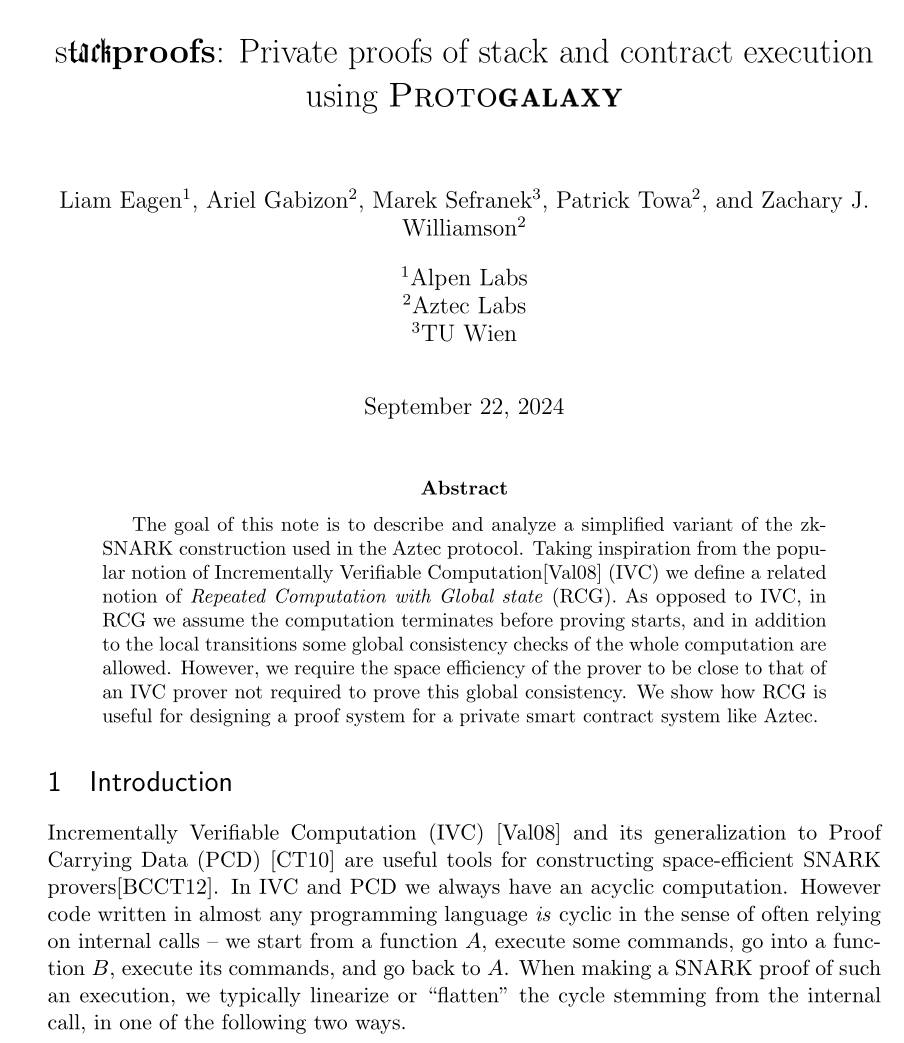
\includegraphics[width=260pt]{stackproofs.png}
\end{figure}
\end{frame}
% 
\end{document}
